\documentclass[
    table,
    10pt,
    twoside,
    a4paper,
    italian
]{book}

\PassOptionsToPackage{dvipsnames}{xcolor} % colori PDF/A

\usepackage{colorprofiles}
% PDF/A
% validate in https://www.pdf-online.com/osa/validate.aspx
\usepackage[a-1a,mathxmp]{pdfx}[2018/12/22]
\usepackage[T1]{fontenc}
\usepackage[utf8]{inputenc}
\usepackage[italian]{babel}
\usepackage{bookmark}
\usepackage{caption}
\usepackage{comment}
\usepackage{chngpage, calc} % centra il frontespizio
\usepackage{emptypage} % pagine vuote senza testatina e piede di pagina
\usepackage{epigraph} % per epigrafi
\usepackage{indentfirst} % rientra il primo paragrafo di ogni sezione
\usepackage{graphicx} % immagini
\usepackage[pdfa]{hyperref} % collegamenti ipertestuali
\usepackage{mparhack,relsize}  % finezze tipografiche
\usepackage{nameref} % visualizza nome dei riferimenti
\usepackage[font=small]{quoting} % citazioni
\usepackage{subfig} % sottofigure, sottotabelle
\usepackage[italian]{varioref} % riferimenti completi della pagina
\usepackage{longtable} % tabelle su più pagine
\usepackage[toc, acronym, automake]{glossaries}
\usepackage[backend=biber, style=verbose-ibid, hyperref, backref]{biblatex}
\usepackage{lmodern}
\usepackage[top=2.75cm, bottom=2.75cm, right=3cm, left=3.75cm]{geometry} % 1in+17pt+0.6cm
\usepackage{fancyhdr}
\usepackage{lipsum}
\usepackage{graphicx}
\usepackage{float}
\usepackage{setspace}
\usepackage{titlesec}
\usepackage{minted} % https://it.overleaf.com/learn/latex/Code_Highlighting_with_minted
\usepackage{xcolor}
\usepackage{csquotes} % gestisce automaticamente i caratteri (")
\usepackage{etoolbox}
\usepackage[table,xcdraw]{xcolor}
\usepackage{changepage}
% Load variables
\newcommand{\myUni}{Università degli Studi di Padova}
\newcommand{\myDepartment}{Dipartimento di Matematica ``Tullio Levi-Civita''}
\newcommand{\myFaculty}{Corso di Laurea in Informatica}
\newcommand{\myTitle}{Una libreria per la visualizzazione di dashboard dinamiche.​}
\newcommand{\myDegree}{Tesi di Laurea Triennale}
\newcommand{\profTitle}{Prof.}
\newcommand{\myProf}{Baldan Paolo}
\newcommand{\graduateTitle}{Laureando}
\newcommand{\myName}{Bresolin Gianluca}
\newcommand{\myStudentID}{2034316}
\newcommand{\myAA}{2023-2024}
\newcommand{\myLocation}{Padova}
\newcommand{\myTime}{Luglio 2024}
% Acronyms

% Glossary

\newglossaryentrywithacronym{SDK}{SDK}{Software Development Kit}{
    Un \textit{Software Development Kit (SDK)} è un insieme di strumenti di sviluppo software riuniti in un unico pacchetto installabile.
    Gli SDK sono progettati per semplificare il processo di sviluppo di applicazioni, fornendo librerie, strumenti di sviluppo, documentazione e esempi di codice
}

\newglossaryentrywithacronym{FCP}{FCP}{First Contentful Paint}{
    Il \textit{First Contentful Paint (FCP)} è una metrica che misura il tempo dal momento in cui una pagina inizia il caricamento fino al momento in cui qualsiasi parte
    del contenuto della pagina viene resa visibile sullo schermo
}

\newglossaryentrywithacronym{SVG}{SVG}{Scalable Vector Graphics}{
    L'\textit{SVG (Scalable Vector Graphics)} è un formato di file basato su \textit{XML} per descrivere immagini vettoriali bidimensionali.
    Questo formato permette la rappresentazione di grafica vettoriale con alta precisione, consentendo lo zoom e il ridimensionamento senza perdita di qualità.
    Gli SVG sono utilizzati ampiamente nel \textit{web design} e nelle applicazioni grafiche grazie alla loro scalabilità e al supporto per interattività e animazioni tramite script e fogli di stile
}

\newglossaryentrywithacronym{API}{API}{Application Programming Interface}{
    Un'\textit{API (Application Programming Interface)} è un insieme di definizioni e protocolli che permettono a diversi software di comunicare tra loro.
    Le API forniscono un'interfaccia standardizzata che consente agli sviluppatori di accedere a funzionalità e servizi di un altro software, sistema operativo, libreria o
    framework senza conoscere i dettagli della loro implementazione
}

\newglossaryentrywithacronym{TTI}{TTI}{Time to Interactive}{
    Il \textit{Time to Interactive (TTI)} è una metrica che misura il tempo necessario affinché una pagina web diventi completamente interattiva, cioè quando è possibile
    interagire con tutti gli elementi principali della pagina senza ritardi significativi
}

\newglossaryentry{open-source}{
    name={Open-Source},
    text={open-source},
    sort=open-source,
    description={Il termine \textit{open-source} si riferisce a un tipo di software il cui codice sorgente è disponibile per l'uso, la modifica e la distribuzione da parte di chiunque.
            Questo modello promuove la collaborazione e la trasparenza nello sviluppo software}
}

\newglossaryentry{refactoring}{
    name={Refactoring},
    text={refactoring},
    sort=refactoring,
    description={Il refactoring è il processo di ristrutturazione del codice sorgente di un programma senza modificarne il comportamento esterno.
            L'obiettivo è migliorare la leggibilità, la manutenibilità e la riduzione della complessità del codice}
}

\newglossaryentry{package}{
    name={Package},
    text={package},
    sort=package,
    description={Un \textit{package} è un insieme di moduli o classi che vengono raggruppati insieme e distribuiti come una singola unità.
            I pacchetti facilitano la gestione e la distribuzione del software, includendo tutte le dipendenze necessarie}
}

\newglossaryentry{bundle}{
    name={Bundle},
    text={bundle},
    sort=bundle,
    description={Un \textit{bundle} è un pacchetto che contiene diversi file e risorse che vengono aggregati insieme per essere distribuiti come un'unica unità.
            In ambito web, un \textit{bundle} può includere file \textit{JavaScript}, \textit{CSS} e immagini}
}

\newglossaryentry{backend}{
    name={Backend},
    text={backend},
    sort=backend,
    description={Il \textit{backend} si riferisce alla parte server di un'applicazione, che gestisce la logica, le operazioni di database, l'autenticazione degli utenti e
            altre funzionalità che non sono visibili direttamente dall'utente finale}
}

\newglossaryentry{responsive}{
    name={Responsive},
    text={responsive},
    sort=responsive,
    description={Il termine \textit{responsive} si riferisce a un design che è in grado di adattarsi a diverse dimensioni dello schermo e dispositivi,
            offrendo un'esperienza utente ottimale, indipendentemente dal dispositivo utilizzato}
}

\newglossaryentry{rendering}{
    name={Rendering},
    text={rendering},
    sort=rendering,
    description={Il rendering è il processo di generazione di un'immagine o di una visualizzazione a partire da un modello o da un insieme di dati.
            In ambito web, il rendering si riferisce alla trasformazione del codice \textit{HTML, CSS} e \textit{JavaScript} in una pagina web visibile e interattiva.
            Il rendering può essere eseguito lato \textit{client}, nel \textit{browser},
            o lato \textit{server}, prima che la pagina venga inviata al \textit{client}}
}

\newglossaryentry{runtime}{
    name={Runtime},
    text={runtime},
    sort=runtime,
    description={Il \textit{runtime} si riferisce al periodo di tempo durante il quale un programma è in esecuzione. Il termine viene anche utilizzato per indicare un ambiente o
            una libreria che supporta l'esecuzione di un programma, fornendo servizi come la gestione della memoria e l'esecuzione del codice}
}

\newglossaryentry{super-set}{
    name={Super-Set},
    text={super-set},
    sort=super-set,
    description={Un super-set è un insieme che contiene tutti gli elementi di un altro insieme, detto sottoinsieme. Nel contesto della programmazione, un linguaggio o un \textit{framework}
            può essere considerato un \textit{super-set} se include tutte le funzionalità di un altro linguaggio o \textit{framework}, aggiungendo ulteriori caratteristiche e capacità.}
}

\newglossaryentry{peerdependency}{
    name={Peer Dependency},
    text={peer-dependency},
    sort=peerdependency,
    description={Una \textit{peer dependency} è una dipendenza di un modulo che non viene installata automaticamente, ma che deve essere fornita dall'ambiente in cui il modulo stesso è eseguito.
            Questo tipo di dipendenza è utilizzato per garantire che i moduli condividano una singola istanza di una libreria comune, evitando problemi di incompatibilità e ridondanza.}
}

\newglossaryentry{bundler}{
    name={Bundler},
    text={bundler},
    sort=bundler,
    description={Un \textit{bundler} è uno strumento utilizzato nello sviluppo web per combinare diversi file e risorse, come \textit{JavaScript}, \textit{CSS} e immagini, in un unico
            file o in un insieme di file più ridotto. Questo processo migliora l'efficienza del caricamento delle pagine web riducendo il numero di richieste HTTP necessarie}
}

\newglossaryentry{tree-shaking}{
    name={Tree-Shaking},
    text={tree-shaking},
    sort=tree-shaking,
    description={Il \textit{tree-shaking} è una tecnica di ottimizzazione del codice utilizzata dai \textit{bundler} per rimuovere codice inutilizzato dai file JavaScript. Questo processo
            analizza le dipendenze del codice per identificare e eliminare le parti che non sono effettivamente utilizzate, riducendo la dimensione finale del \textit{bundle} e migliorando le
            prestazioni delle applicazioni web}
}

\newglossaryentry{memoizzato}{
    name={Memoizzato},
    text={memoizzato},
    sort=memoizzato,
    description={Il termine \textit{memoizzato} si riferisce a una tecnica di ottimizzazione che memorizza il risultato di una funzione o di un calcolo in modo da poterlo riutilizzare
            in seguito senza doverlo ricalcolare. Questo approccio migliora le prestazioni dell'applicazione riducendo il tempo di esecuzione e l'utilizzo delle risorse}
}

\newglossaryentry{frontend}{
    name={Frontend},
    text={frontend},
    sort=frontend,
    description={Il \textit{frontend} si riferisce alla parte visibile di un'applicazione, che interagisce direttamente con l'utente finale. Questa parte dell'applicazione gestisce l'interfaccia
            utente, la presentazione dei dati e le interazioni con l'utente}
}

\newglossaryentry{repository}{
    name={Repository},
    text={repository},
    sort=repository,
    description={Un \textit{repository} è un archivio centralizzato e strutturato per la conservazione, la gestione e il controllo di versioni di codice sorgente, documentazione e altri file correlati
            a un progetto software. I repository possono essere ospitati su server locali o remoti e sono spesso gestiti tramite sistemi di controllo versione, consentendo agli sviluppatori di collaborare,
            tracciare modifiche, gestire diramazioni (\textit{branch}) e fusioni (\textit{merge}), mantenendo una cronologia accurata dello sviluppo del software}
}

\newglossaryentry{framework}{
    name={Framework},
    text={framework},
    sort=framework,
    description={Un \textit{framework} è un insieme di librerie, strumenti e linee guida che forniscono una struttura e un'infrastruttura per lo sviluppo di applicazioni software.
            I \textit{framework} semplificano il processo di sviluppo fornendo funzionalità comuni, standardizzando le pratiche di programmazione e riducendo la complessità del codice}
}

\newglossaryentry{memory leak}{
    name={Memory Leak},
    text={memory leak},
    sort=memoryleak,
    description={Un \textit{memory leak} (perdita di memoria) è una condizione anomala in cui un programma software, durante la sua esecuzione, non rilascia correttamente la memoria che ha allocato.
            Questo comportamento porta ad un utilizzo inefficiente della memoria disponibile, riducendone progressivamente la quantità fino a potenzialmente esaurire tutte le risorse di memoria del sistema.
            I \textit{memory leak} sono spesso causati da errori di programmazione, come la mancata deallocazione di memoria dinamica o riferimenti pendenti a oggetti non più utilizzati}
}

\newglossaryentry{mock}{
    name={Mock},
    text={mock},
    sort=mock,
    description={Un \textit{mock} è un oggetto simulato o fittizio che viene utilizzato al posto di un oggetto o una funzione reale durante i test software. I \textit{mock} vengono utilizzati per simulare il comportamento
            di un oggetto o funzione reale, consentendo ai test di verificare il funzionamento del codice in modo controllato e prevedibile, limitando le responsabilità testate alle sole logiche specifiche}
}

\newglossaryentry{munging}{
    name={Munging},
    text={munging},
    sort=munging,
    description={Il \textit{munging} è una tecnica di trasformazione dei dati che modifica o oscura i dati in modo da renderli irriconoscibili o incomprensibili per chi non è autorizzato a visualizzarli.
            Il \textit{munging} viene spesso utilizzato per proteggere i dati sensibili o per nascondere informazioni personali, come indirizzi email o numeri di telefono, sostituendo i caratteri con simboli o codici.
            Questa tecnica viene inoltre utilizzata per ottimizzare il codice sorgente, riducendo la dimensione dei file}
}

% Define custom colors
\definecolor{hyperColor}{HTML}{0B3EE3}
\definecolor{tableGray}{HTML}{F5F5F7}

% Set line height
\linespread{1.2}

% Custom hyphenation rules
\hyphenation {
    e-sem-pio
    ex-am-ple
}

% Images path
\graphicspath{{img/}}

% Force page color, as some editors set a grayish color as default
\pagecolor{white}

% Better spacing for footnotes
\setlength{\skip\footins}{5mm}
\setlength{\footnotesep}{5mm}

\setlength{\headheight}{14.5pt}
\addtolength{\topmargin}{-2.45pt}

% Add a subscript G to a glossary entry
\newcommand{\glox}{\textsubscript{\textbf{\textit{G }}}}

% If the subscript G is followed by a punctuation character, or anything else, you need to use \gloxspacing to prevent rendering issues, where the characters collide. Example in Chapter 7
\newcommand{\gloxspacing}{\hspace{-0.3em}}

% Improvements the paragraph command
\titleformat{\paragraph}
{\normalfont\normalsize\bfseries}{\theparagraph}{1em}{}
\titlespacing*{\paragraph}
{0pt}{3.25ex plus 1ex minus .2ex}{1.5ex plus .2ex}

% Define use case environment
\newcounter{usecasecounter} % define a counter
\setcounter{usecasecounter}{0} % set the counter to some initial value
% Parameters
% #1: ID
% #2: Nome
\newenvironment{usecase}[2]{
    \renewcommand{\theusecasecounter}{\usecasename #1}  % this is where the display of the counter is overwritten/modified
    \refstepcounter{usecasecounter} % increment counter
    \vspace{2em}
    \par \noindent % start new paragraph
    {\normalsize \textbf{\usecasename #1: #2}} % display the title before the content of the environment is displayed
    \vspace{.5em}
}{
    \medskip
}
\newcommand{\usecasename}{UC}
\newcommand{\usecaseactors}[1]{\textbf{\\Attori Principali:} #1}
\newcommand{\usecasepre}[1]{\textbf{\\Precondizioni:} #1}
\newcommand{\usecasedesc}[1]{\textbf{\\Descrizione:} #1}
\newcommand{\usecasepost}[1]{\textbf{\\Postcondizioni:} #1}
\newcommand{\usecasealt}[1]{\textbf{\\Scenario Alternativo:} #1}

% Define risks environment
\newcounter{riskcounter} % define a counter
\setcounter{riskcounter}{0} % set the counter to some initial value
% Parameters
% #1: Title
\newenvironment{risk}[1]{
    \refstepcounter{riskcounter} % increment counter
    \par \noindent % start new paragraph
    \textbf{\arabic{riskcounter}. #1} % display the title before the content of the environment is displayed
}{
    \par\medskip
}
\newcommand{\riskname}{Rischio}
\newcommand{\riskdescription}[1]{\textbf{\\Descrizione:} #1.}
\newcommand{\risksolution}[1]{\textbf{\\Soluzione:} #1.}

% Apply fancy styling to pages
\pagestyle{fancy}
\fancyhf{}
\fancyhead[L]{\leftmark} % Places Chapter N. Chatper title on the top left
\fancyfoot[C]{\thepage} % Page number in the center of the footer

% Adds a blank page while increasing the page number
\newcommand\blankpage{
    \clearpage
    \begingroup
    \null
    \thispagestyle{empty}
    \hypersetup{pageanchor=false}
    \clearpage
    \endgroup
}

% Increase page numbering
\newcommand\increasepagenumbering{
    \addtocounter{page}{+1}
}

% Make glossaries and bibliography
\makeglossaries
\bibliography{references/bibliography}
\defbibheading{bibliography} {
    \cleardoublepage
    \phantomsection
    \addcontentsline{toc}{chapter}{\bibname}
    \chapter*{\bibname\markboth{\bibname}{\bibname}}
}

% Code blocks handling w/ table of codes
\makeatletter
\ifdefined\NR@chapter
    \expandafter\@firstoftwo
\else
    \expandafter\@secondoftwo
\fi{\patchcmd\NR@chapter}{\patchcmd\@chapter}
{\addtocontents{lot}{\protect\addvspace{10\p@}}}
{\addtocontents{lot}{\protect\addvspace{10\p@}}%
\addtocontents{lol}{\protect\addvspace{10\p@}}}
{}{}
\makeatother

\renewcommand\listingscaption{Codice}
\renewcommand\listoflistingscaption{Elenco dei codici sorgenti}
\counterwithin*{listing}{chapter}
\renewcommand\thelisting{\thechapter.\arabic{listing}}

% Set up hyperlinks
\hypersetup{
    colorlinks=true,
    linktocpage=true,
    pdfstartpage=1,
    pdfstartview=,
    breaklinks=true,
    pdfpagemode=UseNone,
    pageanchor=true,
    pdfpagemode=UseOutlines,
    plainpages=false,
    bookmarksnumbered,
    bookmarksopen=true,
    bookmarksopenlevel=1,
    hypertexnames=true,
    pdfhighlight=/O,
    allcolors = hyperColor
}

% Set up captions
\captionsetup{
    tableposition=top,
    figureposition=bottom,
    font=small,
    format=hang,
    labelfont=bf
}

\date{}

\hypersetup{pdfstartview=}
\begin{document}
\frontmatter
\begin{titlepage}
    \begin{center}
        \begin{Large}
            \textbf{\myUni}\\
        \end{Large}

        \vspace{5pt}

        \begin{large}
            \textsc{\myDepartment}\\
        \end{large}

        \vspace{5pt}

        \begin{large}
            \textsc{\myFaculty}\\
        \end{large}

        \vspace{25pt}
        
        \begin{figure}[htbp]
            \centering
            
\includegraphics[alt={Emblema dell'Università degli Studi di Padova}, height=6cm]{img/logo_unipd.jpeg}
        \end{figure}

        
        \begin{Large}
            \textbf{\myTitle}\\
        \end{Large}

        \vspace{5pt}

        \begin{large}
            \textit{\myDegree}\\
        \end{large}

        \vspace{50pt}
        
        \begin{normalsize}
            \begin{flushleft}
                \textit{Relatore}\\
                \profTitle\ \myProf
            \end{flushleft}

            \vspace{-48pt}
            
            \begin{flushright}
                \textit{\graduateTitle}\\
                \myName\\
                Matricola \myStudentID
            \end{flushright}
        \end{normalsize}

        \vspace*{\fill}
        
        \line(1, 0){338} \\
        \begin{normalsize}
            \textsc{Anno Accademico \myAA}
        \end{normalsize}
    \end{center}
\end{titlepage}

\increasepagenumbering % increase the page numbrering by 1, in order to cout the frontispiece
\clearpage
\phantomsection
\thispagestyle{empty}
\hfill
\vfill

{\small\noindent\textcopyright\ \myName, \myTime. Tutti i diritti riservati. \myDegree: ``\textit{\myTitle}'', \myUni, \myDepartment.}
\cleardoublepage
\phantomsection
\pdfbookmark{Ringraziamenti}{Ringraziamenti}

\begin{flushright}{
        \slshape
        ``''} \\
    \medskip
    --- .
\end{flushright}

\begingroup
\let\clearpage\relax
\let\cleardoublepage\relax
\let\cleardoublepage\relax

\chapter*{Ringraziamenti}

\noindent Desidero esprimere la mia gratitudine al professor \myProf, mio relatore, per l'aiuto e il sostegno che mi ha dato durante la stesura dell'elaborato.

\vspace{0.35cm}

\noindent Vorrei anche ringraziare, con affetto, i miei genitori per il loro sostegno, il grande aiuto e la loro presenza in ogni momento durante gli anni di studio.

\vspace{0.35cm}

\noindent Desidero poi ringraziare i miei amici per i bellissimi anni trascorsi insieme e le mille avventure vissute.

\vspace{0.75cm}

\noindent{\myLocation, \myTime}
\hfill \textit{\myName}

\endgroup

\cleardoublepage
\phantomsection
\pdfbookmark{Compendio}{Compendio}
\begingroup
\let\clearpage\relax
\let\cleardoublepage\relax
\chapter*{Sommario}

Il presente documento descrive il lavoro svolto durante il periodo di stage, \lipsum[1]

\endgroup
\vfill

\cleardoublepage
\pdfbookmark{\contentsname}{tableofcontents}
\setcounter{secnumdepth}{5}
\setcounter{tocdepth}{5}     

\tableofcontents
\clearpage

\begingroup
    \let\clearpage\relax
    \let\cleardoublepage\relax
    \let\cleardoublepage\relax

    % Figures list
    \phantomsection
    \pdfbookmark{\listfigurename}{lof}
    \listoffigures
    \vspace*{8ex}

    % Tables list
    \phantomsection
    \pdfbookmark{\listtablename}{lot}
    \listoftables
\endgroup

\begingroup
    % Code list
    \phantomsection
    \pdfbookmark{\listoflistingscaption}{lol}
    \listoflistings
\endgroup

\cleardoublepage
\printglossary[type=\acronymtype, title=Acronimi e abbreviazioni, toctitle=Acronimi e abbreviazioni]
\printglossary[type=main, title=Glossario, toctitle=Glossario]
\blankpage % example of a blank page that also increases the page couter by 1

\mainmatter
\chapter{Introduzione}
\label{chap:introduzione}

% * INTRODUZIONE

% - Breve descrizione del progetto
% - Principali problematiche
% - Soluzione scelta
% - Strumenti utilizzati
% - Descrizione del prodotto ottenuto
% - Struttura del resto della relazione

\section{L'azienda}
Lo stage è stato svolto presso l'azienda Datasoil S.r.l. situata nei dintorni della stazione ferroviaria di Padova.
Fondata nel XXXX, Datasoil S.r.l. è un'azienda di prodotto che si dedica allo sviluppo di piattaforme per l'industria 4.0,
smart building e smart city.
L'obiettivo dell'azienda è integrare informazioni ed eventi provenienti dai vari livelli aziendali per creare insight proattivi
in tempo reale, garantendo che le informazioni corrette raggiungano le persone giuste al momento più opportuno.
Il punto di partenza è la spazialità aziendale e tutti gli asset che risiedono all'interno di essa, da cui
provengono tutti i dati che vengono analizzati trasversalmente grazie a sempre più persone e dispositivi connessi.
Da qui il nome dell'azienda, Datasoil: fare le informazioni da questo suolo fertile di dati da cui siamo circondati.

\begin{figure}[H]
      \centering
      
\includegraphics[alt={Logo Datasoil S.r.l.}, width=0.25\columnwidth]{img/datasoil_logo.jpg}
      \caption{Logo Datasoil S.r.l.}
      \label{fig:datasoil}
\end{figure}

\section{L'idea}
\subsection{Il contesto applicativo}
L'azienda Datasoil S.r.l., essendo un'azienda di prodotto, nasce con l'idea di proporre servizi di monitoraggio e controllo
di impianti industriali, smart building e smart city, offrendo come principale prodotto la piattaforma SYN.

\begin{figure}[H]
      \centering
      
\includegraphics[alt={Logo SYN}, width=0.25\columnwidth]{img/syn_logo.jpg}
      \caption{Logo SYN}
      \label{fig:syn}
\end{figure}

SYN è una piattaforma di monitoraggio e controllo di impianti industriali che raccoglie dati da sensori e dispositivi
distribuiti all'interno di un impianto o su più stabilimenti, permettendo di visualizzare in tempo reale lo stato di
funzionamento dei vari asset, di analizzare i dati raccolti e di attuare azioni di controllo o segnalazione tramite
ticketing. All'interno della piattaforma, a seconda dei piani attivati dal cliente, è possibile visualizzare dashboard dinamiche
in merito ad informazioni filtrate e aggiornate live, permettendo di raggiungere una panoramica completa dello stato dei vari
asset monitorati in modo rapido, intuitivo ed efficace, grazie all'utilizzo di molteplici grafici e widget.

\subsection{Il progetto}
Il progetto svolto durante lo stage consiste nello sviluppo di una libreria TypeScript di componenti per la creazione di dashboard dinamiche.
Questo è stato realizzato tramite il refactoring e l'ottimizzazione di un tool grafico preesistente, integrato nei vari prodotti di Datasoil S.r.l.,
tra cui \textit{SYN}. La libreria è stata implementata a partire da una libreria open-source utilizzata in \textit{Redash},
una piattaforma per la creazione di dashboard dinamiche tramite interrogazioni sulle fonti di dati configurate all'interno del servizio. \newline
L'esigenza di tale progetto nasce dalla necessità da parte di Datasoil S.r.l. di avere una libreria grafica aggiornata alle versioni
correnti delle dipendenze utilizzate, raggiungendo una maggior performance e una maggiore manutenibilità del codice rispetto alla versione
preesistente, riducendo dove possibile le dipendenze esterne e introducendo migliorie grafiche e funzionali.

\section{Principali problematiche}
Durante l'analisi iniziale della libreria preesistente in uso all'interno dei prodotti di Datasoil S.r.l., sono emerse a fronte di una
revisione del codice sorgente alcune problematiche legate alla manutenibilità e alla performance del tool grafico.

\subsection{Dipendenze obsolete}
La libreria preesistente utilizzava versioni obsolete delle dipendenze esterne, con conseguente rallentamento delle prestazioni in termini
di utilizzo di spazio e di tempo di caricamente delle risorse, data l'assenza di ottimizzazioni e di aggiornamenti del codice sorgente. \newline
Essendo inoltre la libreria preesistente basata su una versione della piattaforma \textit{Redash}, i moduli utilizzati il più delle volte
rappresentavono alternative a quelli già utilizzati all'interno dei prodotti Datasoil S.r.l., creando una dipendenze non necessarie che
causavano un aumento delle dimensioni del SDK utilizzato per la creazione delle dashboard.

\subsection{Manutenibilità del codice}
Il codice sorgente della libreria preesistente, essendo stato sviluppato a fronte di una esigenza specifica dell'azienda Datasoil S.r.l.,
risultava essere poco manutenibile e assente di documentazione. \newline
Inoltre, la libreria utilizzata da \textit{Redash}, inizialmente era stata sviluppata in JavaScript, subendo solo successivamente un
refactoring in TypeScript: questo refactoring non è però avvenuto con l'introduzione di interfacce e tipi, bensì con la semplice aggiunta
di tipi \textit{any} per le variabili e i parametri delle funzioni, rendendo il codice poco leggibile e difficile da mantenere.

\subsection{Componenti inutilizzate}
In quanto la libreria preesistente fosse realizzata a partire dal modulo utilizzato dalla piattaforma \textit{Redash}, non tutti i componenti presenti
in essa trovavano utilizzo all'interno dei prodotti realizzati da Datasoil S.r.l.: questo in gran parte era dovuto da una offerta di grafici inopportuni
per quello che è il contesto applicativo dell'azienda.

\subsection{Assenza di funzionalità}
La libreria preesistente non soddisfaceva pienamente le esigenze dei clienti di Datasoil S.r.l., mancando di alcune funzionalità fondamentali.
Questa limitazione ha reso necessario un intervento di refactoring per colmare le lacune e migliorare le prestazioni complessive.

\section{Soluzione scelte}
Per risolvere le problematiche emerse durante l'analisi iniziale della libreria preesistente, si è optato per il refactoring e l'ottimizzazione
del codice sorgente, individuando le soluzioni presentate di seguito.

\subsection{Aggiornamento delle dipendenze}
Per risolvere il problema delle dipendenze obsolete, è stata effettuata un'analisi delle versioni correnti delle dipendenze utilizzate all'interno della libreria,
verificando che le funzionalità utilizzate non fossero deprecate o rimosse, procedendo con l'eventuale refactoring ad un codice compatibile, che inoltre tenesse conto
delle nuove funzionalità introdotte nelle versioni più recenti. \newline
Grazie ad uno studio accurato delle librerie utilizzate nei prodotti Datasoil S.r.l., è stato possibile sostituire con librerie equivalenti dipendenze preesistenti,
riducendo così l'onere di utilizzo dell'SDK all'interno dei prodotti aziendali.

\subsection{Introduzione di interfacce e tipi}
Al fine di migliorare la manutenibilità e la comprensione del codice sorgente, è stato svolto un lavoro di introduzione di interfacce e tipi per le variabili e i parametri
delle funzioni, in modo da rendere il codice più leggibile e permettere controlli statici sul codice sorgente. \newline
Questo lavoro ha permesso di ridurre la presenza di tipi \textit{any} all'interno del codice sorgente, garantendo una maggiore sicurezza e affidabilità del prodotto finale.

\subsection{Refactoring del codice}
Per migliorare la comprensione e la manutenibilità del codice sorgente, è stato intrapreso un lavoro di refactoring su alcune porzioni della libreria preesistente.
Questo intervento ha comportato la riscrittura di diverse funzioni e la rimozione di componenti minori utilizzate per eseguire funzionalità semplici, attraverso un codice
più leggibile e immediato, eliminando complessità superflue e mantenendo l'efficacia nell'implementazione di operazioni elementari.

\subsection{Rimozione di componenti inutilizzate}
In merito alla presenza di componenti inutilizzate all'interno della libreria preesistente, è stata effettuata un'accurata analisi delle componenti presenti, selezionando
quelle che non trovavano un diretto utilizzo all'interno dei prodotti Datasoil S.r.l. e procedendo con la loro rimozione. \newline
Questo lavoro ha permesso di ridurre le dimensioni del codice sorgente e di migliorare le prestazioni complessive della libreria, diminuendo inoltre il numero di dipendenze
esterne richiesto per il corretto funzionamento dell'SDK prodotto.

\subsection{Implementazione di nuove funzionalità}
Per colmare le lacune riscontrate nella libreria preesistente in merito all'assenza di alcune funzionalità richieste dai clienti di Datasoil S.r.l. all'interno dei prodotti forniti,
è stato condotto un lavoro di implementazione di nuove funzionalità. \newline
In questo processo, si è cercato preferibilmente di utilizzare dipendenze esterne già esistenti o che fossero compatibili con il contesto applicativo dell'azienda. Qualora ciò non
fosse stato possibile, sono state introdotte nuove dipendenze esterne selezionate a seguito di analisi dettagliata che tenesse conto delle implicazioni in termini di dimensioni
finali dell'SDK prodotto.


\section{Descrizione del prodotto ottenuto}

\section{Organizzazione del testo}
Nel presente capitolo viene presentata l'introduzione della tesi, fornendo una panoramica sull'azienda, sul contesto applicativo,
sul progetto e sul prodotto portato a termine durante lo svolgimento dello stage. \newline
In seguito il documento presenterà la seguente organizzazione:

\begin{description}
\item[{\hyperref[chap:analisi-requisiti]{Analisi dei requisiti}}] descrive la fase di analisi dei requisiti che è stata
svolta dall'azienda antecedentemente all'inizio dell'attività di stage, in modo da permettere una comprensione più profonda
di quelle che sono le necessità da soddisfare e gli obiettivi da raggiungere all'interno di questo progetto;

\item[{\hyperref[chap:descrizione-stage]{Progettazione}}] illustra l'attività di progettazione che è stata svolta in vista dell'implementazione
dei grafici prodotti, definendo le tecnologie e le soluzioni implementative che sono state attuate durante la successiva attività di codifica;

\item[{\hyperref[chap:analisi-requisiti]{Realizzazione e Testing}}] approfondisce l'attività di codifica delle componenti grafiche presentate
all'interno della libreria implementata e dei relativi test effettuati per garantire la qualità e la funzionalità del prodotto finale;

\item[{\hyperref[chap:conclusioni]{Conclusioni}}] presentano un epilogo del progetto svolto, includendo una valutazione oggettiva
degli strumenti utilizzati e una riflessione sui possibili punti di insoddisfazione e dei relativi miglioramenti applicabili al prodotto realizzato.
La sezione infine si conclude con proposte per future estensioni e sviluppi del progetto.

In merito alla stesura del testo, all'interno del presente documento sono state adottate le seguenti convenzioni tipografiche:
\begin{itemize}
      \item gli acronimi, le abbreviazioni e i termini ambigui o di uso non comune menzionati vengono definiti nel glossario, situato alla fine del presente documento;
      \item per la prima occorrenza dei termini riportati nel glossario viene utilizzata la seguente nomenclatura: \textit{parola}\glox\gloxspacing;
      \item i termini in lingua straniera o facenti parti del gergo tecnico sono evidenziati con il carattere \textit{corsivo}.
\end{itemize}


\newpage
\chapter{Analisi dei requisiti}
\label{chap:analisi-requisiti}
Nel seguente capito verrà descritta l'attività di analisi dei requisiti inerente al progetto di stage. \newline
In quanto l'SDK in questione è uno strumento live sui diversi prodotti Datasoil S.r.l., l'analisi dei requisiti è stata svolta
in fase antecedente all'inizio dello stage da parte del team di sviluppo frontend dell'azienda. \newline
A fronte di tale contesto, nella seguente sezione verranno riportati i requisiti individuati in modo da poter fornire il contesto
necessario alla comprensione del progetto, senza approfondire l'attività di analisi svolta.

\section{Classificazione dei requisiti}
I requisiti presentati all'interno del documento vengono classificati in tre categorie, in base alle esigenze che definiscono, venendo inoltre
associati ad un livello di priorità che ne determina l'obbligatorietà o l'opzionalità. \newline

\newline
Le categorie di classificazione definite all'interno del progetto di stage sono:

\begin{itemize}
    \item[\textbf{F}:] \textit{Funzionale}: il requisito definisce le funzionalità che il sistema deve offrire;
    \item[\textbf{A}:] \textit{Di attributo}: il requisito definisce le caratteristiche che il sistema deve avere;
    \item[\textbf{V}:] \textit{Di vincolo}: il requisito definisce i vincoli che il sistema deve rispettare.
\end{itemize}

\newline
I livelli di priorità definiti all'interno del progetto di stage sono:

\begin{itemize}
    \item[\textbf{O}:] \textit{Obbligatorio}: requisito essenziale al fine di concludere il progetto di stage con successo;
    \item[\textbf{OP}:] \textit{Opzionale}: requisito non essenziale al fine di concludere il progetto di stage con successo, ma che aggiunge valore al prodotto finale.
\end{itemize}

\newline
La nomeclatura utilizzata per la classificazione dei requisiti all'interno del progetto di stage è la seguente:
\begin{itemize}
    \item \textbf{R}: dove R sta per requisito;
    \item \textbf{X.}: dove X indica la categoria di classificazione del requisito;
    \item \textbf{Y.}: dove Y indica il livello di priorità del requisito;
    \item \textbf{Z}: dove Z indica il numero progressivo del requisito. Nel caso di sotto-requisiti, il numero progressivo è composto da due cifre, separate da un punto,
          dove la prima cifra rappresenta il requisito padre e la seconda cifra rappresenta il sotto-requisito.
\end{itemize}

\newpage
\section{Requisiti}

\subsection{Requisiti funzionali}
Nella seguente sezione viene presentata la lista dei requisiti funzionali. \newline

\begin{center}
    \rowcolors{1}{white}{tableGray}
    \begin{longtable}{|p{2.5cm}|p{10cm}|}
        \hline
        \rowcolor{gray!30}
        \textbf{Requisito} & \multicolumn{1}{c|}{\textbf{Descrizione}}                                                          \\
        \hline
        \endfirsthead
        \multicolumn{2}{c}{{\tablename\ \thetable{} -- continua dalla pagina precedente}}                                       \\
        \hline
        \rowcolor{gray!30}
        \textbf{Requisito} & \multicolumn{1}{c|}{\textbf{Descrizione}}                                                          \\
        \endhead
        \hline
        \multicolumn{2}{|r|}{{Continua nella prossima pagina...}}                                                               \\
        \hline
        \endfoot
        \hline
        \endlastfoot
        R.F.O.1            & La libreria deve permettere la visualizzazione di grafici.                                         \\
        \hline
        R.F.O.1.1          & La libreria deve permettere la visualizzazione di grafici a barre (\textit{bar or columns}).       \\
        \hline
        R.F.O.1.2          & La libreria deve permettere la visualizzazione di grafici a torta (\textit{pie}).                  \\
        \hline
        R.F.O.1.3          & La libreria deve permettere la visualizzazione di grafici a scatola (\textit{box-plot}).           \\
        \hline
        R.F.O.1.4          & La libreria deve permettere la visualizzazione di grafici a bolle (\textit{bubbles}).              \\
        \hline
        R.F.O.1.5          & La libreria deve permettere la visualizzazione di grafici a dispersione (\textit{scatter}).        \\
        \hline
        R.F.O.1.6          & La libreria deve permettere la visualizzazione di grafici a mappe di calore (\textit{heatmap}).    \\
        \hline
        R.F.O.2            & La libreria deve permettere la visualizzazione di contatori.                                       \\
        \hline
        R.F.O.2.1          & La libreria deve permettere la visualizzazione di contatori con target.                            \\
        \hline
        R.F.O.2.2          & La libreria deve permettere la visualizzazione di contatori senza target.                          \\
        \hline
        R.F.O.3            & La libreria deve permettere la visualizzazione di tabelle.                                         \\
        \hline
        R.F.O.4            & La libreria deve permettere di zoomare i vari grafici.                                             \\
        \hline
        R.F.O.5            & La libreria deve permettere di effettuare il download in \textit{.png} dei grafici renderizzati.   \\
        \hline
        R.F.O.6            & La libreria deve permettere di effettuare il download in \textit{.csv} delle tabelle visualizzate. \\
        \hline
        R.F.O.7            & I widget renderizzati devono adattarsi alla dimensione del contenitore in modo responsivo.         \\
    \end{longtable}
    \captionof{table}{Tabella del tracciamento dei requisiti funzionali.}
    \label{tab:requisiti_funzionali}
\end{center}

\subsection{Requisiti qualitativi}
Nella seguente sezione viene presentata la lista dei requisiti qualitativi. \newline

\begin{center}
    \rowcolors{1}{white}{tableGray}
    \begin{longtable}{|p{2.5cm}|p{10cm}|}
        \hline
        \rowcolor{gray!30}
        \textbf{Requisito} & \multicolumn{1}{c|}{\textbf{Descrizione}}                                                                                    \\
        \hline
        \endfirsthead
        \multicolumn{2}{c}{{\tablename\ \thetable{} -- continua dalla pagina precedente}}                                                                 \\
        \hline
        \rowcolor{gray!30}
        \textbf{Requisito} & \multicolumn{1}{c|}{\textbf{Descrizione}}                                                                                    \\
        \endhead
        \hline
        \multicolumn{2}{|r|}{{Continua nella prossima pagina...}}                                                                                         \\
        \hline
        \endfoot
        \hline
        \endlastfoot
        \hline
        R.A.O.1            & La libreria deve essere facilmente manutenibile, rispettando le convenzioni di codifica
        attualmente in atto all'interno dell'azienda Datasoil S.r.l.                                                                                      \\
        \hline
        R.A.O.2            & La libreria deve essere performante in termini di velocità di rendering dei widget forniti.                                  \\
        \hline
        R.A.O.3            & La libreria deve essere ottimizzata per richiedere il minor numero di rendering possibili durante l'interazione dell'utente,
        eseguendoli in modo efficiente per minimizzare l'uso delle risorse.                                                                               \\
        \hline
        R.A.O.3            & La libreria deve essere leggera in termini di dimensione di memoria occupata.                                                \\
        \hline
        R.A.O.3.1          & Le dipendenze esterne devono essere ridotte al minimo indispensabile.                                                        \\
        \hline
        R.A.0.3.2          & La libreria deve essere composta esclusivamente da codice effettivamente utilizzato per le funzionalità e i widget resi
        disponibili. Ciò comporta che qualsiasi componente di codice inutilizzata, superflua o non necessaria deve essere identificata e rimossa.         \\
    \end{longtable}
    \captionof{table}{Tabella del tracciamento dei requisiti qualitativi.}
    \label{tab:requisiti_qualitativi}
\end{center}

\subsection{Requisiti di vincolo}
Nella seguente sezione viene presentata la lista dei requisiti di vincolo. \newline

\begin{center}
\rowcolors{1}{white}{tableGray}
\begin{longtable}{|p{2.5cm}|p{10cm}|}
    \hline
    \rowcolor{gray!30}
    \textbf{Requisito} & \multicolumn{1}{c|}{\textbf{Descrizione}}                                                 \\
    \hline
    \endfirsthead
    \multicolumn{2}{c}{{\tablename\ \thetable{} -- continua dalla pagina precedente}}                              \\
    \hline
    \rowcolor{gray!30}
    \textbf{Requisito} & \multicolumn{1}{c|}{\textbf{Descrizione}}                                                 \\
    \endhead
    \hline
    \multicolumn{2}{|r|}{{Continua nella prossima pagina...}}                                                      \\
    \hline
    \endfoot
    \hline
    \endlastfoot
    \hline
    R.V.O.1            & La libreria deve essere sviluppata in \textit{TypeScript}.                                \\
    \hline
    R.V.O.2            & La libreria deve essere sviluppata con \textit{React}.                                    \\
    \hline
    R.V.O.3            & La libreria deve essere sviluppata con l'utilizzo di componenti di \textit{PrimeReact}.   \\
    \hline
    R.V.O.4            & La libreria deve essere sviluppata con l'utilizzo di \textit{PrimeFlex}.                  \\
    \hline
    R.V.O.5            & La libreria deve essere sviluppata con l'utilizzo di \textit{PrimeIcons}.                 \\
    \hline
    R.V.O.6            & Il codice della libreria deve essere formattato mediante l'utilizzo di \textit{Prettier}. \\
\end{longtable}
\captionof{table}{Tabella del tracciamento dei requisiti di vincolo.}
\label{tab:requisiti_vincolo}


\newpage
\chapter{Progettazione}
\label{chap:progettazione}
Nel presente capitolo viene presentata l'attività di progettazione relativa al progetto di stage focalizzato sul refactoring e
sull'ottimizzazione dello SDK impiegato dall'azienda Datasoil S.r.l. per lo sviluppo di dashboard dinamiche.
Verrà analizzato l'approccio adottato per individuare le soluzioni volte al soddisfacimento dei requisiti individuati durante
la fase di analisi dei requisiti, proseguendo con la descrizione dell'architettura progettata per la realizzazione della libreria grafica \textit{viz-lib}
appartenente al development kit, concludendo con la definizione dei tipi e delle interfacce e la progettazione delle singole componenti individuate.

\section{Metodologia di progettazione}
La metodologia di progettazione adottata durante lo svolgimento del progetto di stage ha seguito inizialmente un approccio
\textit{top-down}, che permettesse, attraverso uno studio generale della libreria preesistente e della sua architettura, di individuare
il flusso di dati tra le varie componenti, fornendo una visione globale delle interazioni e delle dipendenze esistenti.
Successivamente, è stato adottato un approccio \textit{bottom-up}, analizzando le singole componenti e le loro funzionalità,
in modo da identificare le possibili ottimizzazioni e le modifiche necessarie per il miglioramento delle prestazioni, della leggibilità e
della manutenibilità del codice.\newline
L'attività di progettazione è stata condotta in collaborazione stretta con il tutor aziendale, il quale ha fornito supporto e orientamento
riguardo alle decisioni progettuali individuate.

\section{Design dell'architettura}
L'architettura progettata per la realizzazione della libreria grafica si basa su un pattern comunemente utilizzato nello sviluppo di packages
di componenti frontend per \textit{React}, ovvero il pattern \textit{Component Library Architecture}: questa architettura si fonda sulla creazione di una libreria di
componenti riutilizzabili, modulari e indipendenti tra loro. \newline
Tale pattern permette di creare l'architettura ideale per librerie che offrono collezioni di componenti riutilizzabili, permettendo e agevolando
la condivisione e il riutilizzo di codice all'interno del progetto, garantendo una maggior manutenibilità del codice. \newline
Il modello proposto prevede la seguente struttura, la quale si riflette nella definizione delle macro-directory all'interno del progetto:
\begin{itemize}
      \item \textbf{components}: directory contenente i componenti della libreria grafica;
      \item \textbf{hooks}: directory contenente i custom hooks utilizzati all'interno della libreria grafica;
      \item \textbf{utils}: directory contenente le funzioni di utilità utilizzate all'interno della libreria grafica;
      \item \textbf{models}: directory contenente le definizioni dei tipi e delle interfacce utilizzate all'interno della libreria grafica;
      \item \textbf{index.ts}: file principale della libreria grafica, contenente l'esportazione di tutti i componenti e le funzioni utilizzate;
      \item \textbf{style.css}: file contenente i fogli di stile globali utilizzati all'interno della libreria grafica.
\end{itemize}
L'entry point della libreria grafica è il file \textit{index.ts}, il quale si occupa di esportare il \textit{Renderer}, il componente principale
della liberia che si occupa di renderizzare il corretto componente a seconda del tipo di visualizzazione richiesto: tali informazioni necessarie
vengono passate come props dalle componenti del modulo \textit{dashboard} che utilizzano il \textit{Renderer}, riducendo così la dipendenza tra le
componenti di librerie differenti, agevolando la manutenibilità e la scalabilità del codice.


\section{Progettazione dei tipi e delle interfacce}
Nella seguente sezione vengono presentati i tipi e le interfacce definiti durante l'attività di progettazione, associati ad una descrizione dettagliata
delle informazioni che rappresentano. \\
La definizione dei tipi e delle interfacce ha costituito un ruolo fondamentale durante l'attività di progettazione, permettendo di raggiungere una maggior
leggibilità e manutenibilità del codice, permettendo di usufruire a pieno dei vantaggi offerti da \textit{TypeScript}. \\
I tipi e le interfacce verranno presentati in ordine alfabetico.

\subsection{ChartBaseVisualizationOptions}
Interfaccia che definisce i tipi dei dati relativi alle opzioni di visualizzazione comuni a tutti i \textit{Chart}.
\begin{minted}{typescript}
export interface ChartBaseVisualizationOptions {
      globalSeriesType: string; 
      sortX: boolean;
      sortY?: boolean;
      legend: {
      enabled: boolean;
      placement: string;
      traceorder: 'grouped'|'normal'|'reversed'|'reversed+grouped';
      };
      xAxis: {
      labels: {
            enabled: boolean;
      };
      type: string;
      title?: {
            text: string;
      };
      };
      yAxis: [
      {
            type: string;
            rangeMax?: number;
            rangeMin?: number;
            title?: {
            text?: string;
            };
      },
      {
            opposite: boolean;
            type: string;
      },
      ];
      alignYAxesAtZero: boolean;
      error_y: {
      type: string;
      visible: boolean;
      };
      series: {
      error_y: {
            type: string;
            visible: boolean;
      };
      stacking: string;
      percentValues?: boolean;
      };
      seriesOptions: {
      [x: string]: any;
      };
      valuesOptions: {
      [x: string]: any;
      };
      columnMapping: { [x: string]: string };
      direction: {
      type: string;
      };
      sizemode: string;
      coefficient: number;
      showDataLabels: boolean;
      numberFormat: string;
      dateTimeFormat: string;
      percentFormat: string;
      textFormat: string;
      missingValuesAsZero: boolean;
      onHover?: () => void;
      onUnHover?: () => void;
      reverseX?: boolean;
      reverseY?: boolean;
      showpoints?: boolean;
      heatMinColor?: string;
      heatMaxColor?: string;
      colorScheme: string | (string | number)[][];
}
\end{minted}
\begin{listing}[H]
      \caption{Definizione dell'interfaccia ChartBaseVisualizationOptions}
      \label{listing:chartBaseVisualizationOptions}
\end{listing}
\begin{itemize}
      \item \textbf{globalSeriesType}: stringa che definisce il tipo di chart da renderizzare. I valori possibili sono i seguenti:
            \textit{area, column, box, bubble, heatmap, line, pie} e \textit{scatter};
      \item \textbf{sortX}: booleano che definisce se ordinare o meno le serie sull'asse delle ascisse;
      \item \textbf{sortY}: booleano che definisce se ordinare o meno le serie sull'asse delle ordinate;
      \item \textbf{legend}: oggetto che definisce le opzioni della legenda del grafico.
            \begin{itemize}
                  \item \textbf{enabled}: booleano che definisce se abilitare o meno la legenda;
                  \item \textbf{placement}: stringa che definisce la posizione della legenda all'interno del grafico;
                  \item \textbf{traceorder}: stringa che definisce l'ordine delle tracce all'interno del grafico.
            \end{itemize}
      \item \textbf{xAxis}: oggetto che definisce le opzioni dell'asse delle ascisse.
            \begin{itemize}
                  \item \textbf{labels}: oggetto che definisce le opzioni delle label dell'asse delle ascisse;
                  \item \textbf{type}: stringa che definisce il tipo di dato visualizzato sull'asse delle ascisse;
                  \item \textbf{title}: oggetto che definisce il titolo dell'asse delle ascisse.
            \end{itemize}
      \item \textbf{yAxis}: array che definisce le opzioni dell'asse delle ordinate. Ogni elemento dell'array è un oggetto che definisce le opzioni per una serie di dati. \newline
            Il primo oggetto definisce i valori per la serie principale:
            \begin{itemize}
                  \item \textbf{type}: stringa che definisce il tipo di dato visualizzato sull'asse delle ordinate;
                  \item \textbf{rangeMax}: numero che definisce il valore massimo dell'asse delle ordinate;
                  \item \textbf{rangeMin}: numero che definisce il valore minimo dell'asse delle ordinate;
                  \item \textbf{title}: oggetto che definisce il titolo dell'asse delle ordinate.
            \end{itemize}
            Il secondo oggetto definisce i valori per la serie secondaria:
            \begin{itemize}
                  \item \textbf{opposite}: booleano che definisce se la serie secondaria è opposta alla serie principale;
                  \item \textbf{type}: stringa che definisce il tipo di dato visualizzato sull'asse delle ordinate.
            \end{itemize}
      \item \textbf{alignYAxesAtZero}: booleano che definisce se allineare le ordinate a zero;
      \item \textbf{error\_y}: oggetto che definisce le opzioni degli errori sull'asse delle ordinate.
            \begin{itemize}
                  \item \textbf{type}: stringa che definisce il tipo di errore;
                  \item \textbf{visible}: booleano che definisce se visualizzare o meno gli errori.
            \end{itemize}
      \item \textbf{series}: oggetto che definisce le opzioni delle serie.
            \begin{itemize}
                  \item \textbf{error\_y}: oggetto che definisce le opzioni degli errori sull'asse delle ordinate;
                  \item \textbf{stacking}: stringa che definisce se le serie sono sovrapposte o impilate;
                  \item \textbf{percentValues}: booleano che definisce se visualizzare i valori in percentuale.
            \end{itemize}
      \item \textbf{seriesOptions}: oggetto che definisce le opzioni delle serie;
      \item \textbf{valuesOptions}: oggetto che definisce le opzioni dei valori;
      \item \textbf{columnMapping}: oggetto che definisce il mapping delle colonne;
      \item \textbf{direction}: oggetto che definisce tramite type la direzione del grafico;
      \item \textbf{sizemode}: stringa che definisce la modalità di dimensionamento;
      \item \textbf{coefficient}: numero che definisce il coefficiente di dimensionamento;
      \item \textbf{showDataLabels}: booleano che definisce se visualizzare o meno le label dei dati;
      \item \textbf{numberFormat}: stringa che definisce il formato dei numeri;
      \item \textbf{dateTimeFormat}: stringa che definisce il formato della data;
      \item \textbf{percentFormat}: stringa che definisce il formato percentuale;
      \item \textbf{textFormat}: stringa che definisce il formato del testo;
      \item \textbf{missingValuesAsZero}: booleano che definisce se i valori mancanti devono essere considerati come zero;
      \item \textbf{onHover}: funzione che definisce l'azione da eseguire al passaggio del mouse;
      \item \textbf{onUnHover}: funzione che definisce l'azione da eseguire al passaggio del mouse;
      \item \textbf{reverseX}: booleano che definisce se invertire l'asse delle ascisse;
      \item \textbf{reverseY}: booleano che definisce se invertire l'asse delle ordinate;
      \item \textbf{showpoints}: booleano che definisce se visualizzare o meno i punti;
      \item \textbf{heatMinColor}: stringa che definisce il colore minimo del grafico heatmap;
      \item \textbf{heatMaxColor}: stringa che definisce il colore massimo del grafico heatmap;
      \item \textbf{colorScheme}: stringa o array che definisce lo schema dei colori del grafico heatmap.
\end{itemize}

\subsection{Column}
Interfaccia che definisce i tipi dei dati relativi alle colonne della tabella.

\begin{minted}{typescript}
export interface Column {
      title: string;
      name: string;
      type: string;
      visible: boolean;
      displayAs: string;
      header?: any;
      alignContent?: string;
      allowHTML?: boolean; 
      allowSearch?: boolean;
      booleanValues?: string[];
      highlightLinks?: boolean;
      imageTitleTemplate?: string;
      imageUrlTemplate?: string;
      imageWidth?: string;
      imageHeight?: string;
      linkOpenInNewTab?: boolean;
      linkTextTemplate?: string;
      linkTitleTemplate?: string;
      linkUrlTemplate?: string;
      numberFormat?: string;
      dateTimeFormat?: string;
      order?: number;
}
\end{minted}
\begin{listing}[H]
      \caption{Definizione dell'interfaccia Column}
      \label{listing:column}
\end{listing}
\begin{itemize}
      \item \textbf{title}: stringa che definisce il titolo della colonna;
      \item \textbf{name}: stringa che definisce il nome della colonna;
      \item \textbf{type}: stringa che definisce il tipo di dato della colonna;
      \item \textbf{visible}: booleano che definisce se la colonna è visibile o meno;
      \item \textbf{displayAs}: stringa che definisce il tipo di visualizzazione della colonna;
      \item \textbf{header}: oggetto che definisce l'header della colonna;
      \item \textbf{alignContent}: stringa che definisce l'allineamento del contenuto della colonna;
      \item \textbf{allowHTML}: booleano che definisce se permettere o meno l'utilizzo di HTML;
      \item \textbf{allowSearch}: booleano che definisce se permettere o meno la ricerca;
      \item \textbf{booleanValues}: array di stringhe che definisce i valori booleani;
      \item \textbf{highlightLinks}: booleano che definisce se evidenziare i link;
      \item \textbf{imageTitleTemplate}: stringa che definisce il template del titolo dell'immagine;
      \item \textbf{imageUrlTemplate}: stringa che definisce il template dell'URL dell'immagine;
      \item \textbf{imageWidth}: stringa che definisce la larghezza dell'immagine;
      \item \textbf{imageHeight}: stringa che definisce l'altezza dell'immagine;
      \item \textbf{linkOpenInNewTab}: booleano che definisce se aprire il link in una nuova scheda;
      \item \textbf{linkTextTemplate}: stringa che definisce il template del testo del link;
      \item \textbf{linkTitleTemplate}: stringa che definisce il template del titolo del link;
      \item \textbf{linkUrlTemplate}: stringa che definisce il template dell'URL del link;
      \item \textbf{numberFormat}: stringa che definisce il formato numerico;
      \item \textbf{dateTimeFormat}: stringa che definisce il formato della data;
      \item \textbf{order}: numero che definisce l'ordine della colonna.
\end{itemize}


\subsection{CounterVisualizationOptions}
Interfaccia che definisce i tipi dei dati relativi alle opzioni di visualizzazione del componente \textit{Counter}.
\begin{listing}[H]
      \begin{minted}{typescript}
      export interface CounterBaseVisualizationOptions {
            counterLabel: string;
            counterColName: string;
            targetColName?: string;
            rowNumber: number;
            targetRowNumber: number;
            countRows?: any;
            stringDecimal: number;
            stringDecChar: string;
            stringThouSep: string;
            tooltipFormat: string;
            stringPrefix?: string;
            stringSuffix?: string;
            formatTargetValue?: boolean;
      }
      \end{minted}
      \caption{Definizione dell'interfaccia CounterVisualizationOptions}
      \label{listing:counterVisualizationOptions}
\end{listing}
\begin{itemize}
      \item \textbf{counterLabel}: stringa che definisce l'etichetta del contatore;
      \item \textbf{counterColName}: stringa che definisce il nome della colonna contenente i valori del contatore;
      \item \textbf{targetColName}: stringa che definisce il nome della colonna contenente il valore target del contatore;
      \item \textbf{rowNumber}: numero che definisce il numero di righe da considerare per il calcolo del contatore;
      \item \textbf{targetRowNumber}: numero che definisce il numero di righe da considerare per il calcolo del valore target;
      \item \textbf{countRows}: oggetto che definisce le righe da considerare per il calcolo del contatore;
      \item \textbf{stringDecimal}: numero che definisce il numero di cifre decimali da visualizzare;
      \item \textbf{stringDecChar}: stringa che definisce il separatore decimale;
      \item \textbf{stringThouSep}: stringa che definisce il separatore delle migliaia;
      \item \textbf{tooltipFormat}: stringa che definisce il formato del tooltip;
      \item \textbf{stringPrefix}: stringa che definisce il prefisso del contatore;
      \item \textbf{stringSuffix}: stringa che definisce il suffisso del contatore;
      \item \textbf{formatTargetValue}: booleano che definisce se formattare o meno il valore target.
\end{itemize}

\subsection{DataLabels}
Interfaccia che definisce i tipi dei dati relativi alle label dei dati utilizzati negli \textit{heatmaps}.

\begin{minted}{typescript}
export interface DataLabels {
  x: any[];
  y: any[];
  mode: string;
  hoverinfo: string;
  showlegend: boolean;
  text: string[];
  textfont: {
    color: string[];
  };
}
\end{minted}
\begin{listing}[H]
      \caption{Definizione dell'interfaccia DataLabels}
      \label{listing:dataLabels}
\end{listing}
\begin{itemize}
      \item \textbf{x}: array che definisce i valori sull'asse delle ascisse;
      \item \textbf{y}: array che definisce i valori sull'asse delle ordinate;
      \item \textbf{mode}: stringa che definisce la modalità;
      \item \textbf{hoverinfo}: stringa che definisce le informazioni del tooltip;
      \item \textbf{showlegend}: booleano che definisce se visualizzare o meno la legenda;
      \item \textbf{text}: array di stringhe che definisce il testo;
      \item \textbf{textfont}: oggetto che definisce le opzioni del font del testo:
            \begin{itemize}
                  \item \textbf{color}: array di stringhe che definisce i colori del font.
            \end{itemize}
\end{itemize}

\subsection{PlotlyOptions}
Interfaccia che definisce i tipi dei dati relativi alle opzioni di visualizzazione di Plotly.
\begin{minted}{typescript}
export interface PlotlyOptions {
  showLink: boolean;
  displaylogo: boolean;
  displayModeBar?: boolean;
  responsive?: boolean;
  autosize?: boolean;
}
\end{minted}
\begin{listing}[H]
      \caption{Definizione dell'interfaccia PlotlyOptions}
      \label{listing:plotlyOptions}
\end{listing}
\begin{itemize}
      \item \textbf{showLink}: booleano che definisce se visualizzare o meno il link;
      \item \textbf{displaylogo}: booleano che definisce se visualizzare o meno il logo;
      \item \textbf{displayModeBar}: booleano che definisce se visualizzare o meno la barra di Plotly;
      \item \textbf{responsive}: booleano che definisce se rendere o meno il grafico responsivo;
      \item \textbf{autosize}: booleano che definisce se adattare o meno la grandezza del grafico.
\end{itemize}

\subsection{RendererProps}
Interfaccia che definisce i tipi dei dati passati alla componenti \textit{Renderer, Counter, Chart} e \textit{Table}.
\begin{listing}[H]
      \begin{minted}{typescript}
      export interface RendererProps {
            type: string;
            visualizationName: string;
            data: {
                  [x: string]: any;
            };
            options: VisualizationOptions;
      }
      \end{minted}
      \caption{Definizione dell'interfaccia RendererProps}
      \label{listing:rendererProps}
\end{listing}
\begin{itemize}
      \item \textbf{type}: stringa che definisce il tipo componente da renderizzazre. Può assumere i seguenti valori: \textit{COUNTER}, \textit{CHART} e \textit{TABLE};
      \item \textbf{visualizationName}: stringa che definisce il titolo di visualizzazione della componente;
      \item \textbf{data}: oggetto che contiene i dati da visualizzare all'interno della componente;
      \item \textbf{options}: oggetto che contiene le opzioni di visualizzazione della componente di tipo \textit{VisualizationOptions}.
\end{itemize}

\subsection{Series}
Interfaccia che definisce i tipi dei dati relativi alle serie rappresentata nel grafico.
\begin{minted}{typescript}
export interface Series {
  name: string;
  type: string;
  data?: any[];
  visible?: boolean;
  values?: number[];
  labels?: string[];
  hole?: number;
  marker?: {
    colors?: string[];
    color?: string; 
    line?: {
      color?: string;
      width?: number;
    };
    size?: number;
    sizemode?: string;
  };
  hoverinfo?: string | boolean;
  text?: any[];
  textinfo?: string;
  textposition?: string;
  textangle?: number;
  textfont?: {
    size?: number;
    color?: string[];
  };
  direction?: string;
  domain?: {
    x: number[];
    y: number[];
  };
  sourceData?: Map<string, any>;
  hoverlabel?: {
    font?: {
      color?: string[];
    };
    bordercolor?: string;
    bgcolor?: string;
  };
  hover?: any[];
  x?: any;
  y?: any;
  z?: any;
  yaxis?: any;
  orientation?: number;
  insidetextfont?: {
    size?: number;
    color?: string;
  };
  error_y?: any;
  offsetgroup?: string;
  mode?: string;
  fill?: string;
  boxpoints?: string;
  jitter?: number;
  pointpos?: number;
  colorscale?: string | (string | number)[][];
  xgap?: number;
  ygap?: number;
}
\end{minted}
\begin{listing}[H]
      \caption{Definizione dell'interfaccia Series}
      \label{listing:series}
\end{listing}
\begin{itemize}
      \item \textbf{name}: stringa che definisce il nome della serie;
      \item \textbf{type}: stringa che definisce il tipo di serie;
      \item \textbf{data}: array che definisce i dati della serie;
      \item \textbf{visible}: booleano che definisce se la serie è visibile o meno;
      \item \textbf{values}: array di numeri che definisce i valori della serie;
      \item \textbf{labels}: array di stringhe che definisce le label della serie;
      \item \textbf{hole}: numero che definisce, nel caso di grafico a torta, il raggio del buco centrale;
      \item \textbf{marker}: oggetto che definisce le opzioni del marker;
      \item \textbf{hoverinfo}: stringa o booleano che definisce le informazioni del tooltip;
      \item \textbf{text}: array che definisce il testo della serie;
      \item \textbf{textinfo}: stringa che definisce le informazioni del testo;
      \item \textbf{textposition}: stringa che definisce la posizione del testo;
      \item \textbf{textangle}: numero che definisce l'angolo del testo;
      \item \textbf{textfont}: oggetto che definisce le opzioni del font del testo;
      \item \textbf{direction}: stringa che definisce la direzione della serie;
      \item \textbf{domain}: oggetto che definisce il dominio della serie;
      \item \textbf{sourceData}: mappa che definisce i dati sorgente;
      \item \textbf{hoverlabel}: oggetto che definisce le opzioni del tooltip;
      \item \textbf{hover}: array che definisce le opzioni del tooltip;
      \item \textbf{x}: array che definisce i valori sull'asse delle ascisse;
      \item \textbf{y}: array che definisce i valori sull'asse delle ordinate;
      \item \textbf{z}: array che definisce i valori sull'asse z;
      \item \textbf{yaxis}: array che definisce i valori sull'asse delle ordinate;
      \item \textbf{orientation}: numero che definisce l'orientamento;
      \item \textbf{insidetextfont}: oggetto che definisce le opzioni del font interno;
      \item \textbf{error\_y}: oggetto che definisce le opzioni degli errori sull'asse delle ordinate;
      \item \textbf{offsetgroup}: stringa che definisce il gruppo di offset;
      \item \textbf{mode}: stringa che definisce la modalità;
      \item \textbf{fill}: stringa che definisce il riempimento;
      \item \textbf{boxpoints}: stringa che definisce i punti del box;
      \item \textbf{jitter}: numero che definisce il jitter;
      \item \textbf{pointpos}: numero che definisce la posizione del punto;
      \item \textbf{colorscale}: stringa o array che definisce lo schema dei colori;
      \item \textbf{xgap}: numero che definisce il gap sull'asse delle ascisse;
      \item \textbf{ygap}: numero che definisce il gap sull'asse delle ordinate.
      \item \textbf{colors}: array di stringhe che definisce i colori del marker;
      \item \textbf{color}: stringa che definisce il colore del marker;
      \item \textbf{line}: oggetto che definisce le opzioni della linea del marker;
      \item \textbf{size}: numero che definisce la grandezza del marker;
      \item \textbf{sizemode}: stringa che definisce la modalità di dimensionamento del marker.
      \item \textbf{font}: oggetto che definisce le opzioni del font del marker;
      \item \textbf{bordercolor}: stringa che definisce il colore del bordo del marker;
      \item \textbf{bgcolor}: stringa che definisce il colore di sfondo del marker.
      \item \textbf{colors}: array di stringhe che definisce i colori delle rappresentazioni (multiple);
      \item \textbf{size}: numero che definisce la grandezza del font.
      \item \textbf{color}: stringa che definisce il colore della rappresentazione (singola).
\end{itemize}


\subsection{TableBaseVisualizationOptions}
Interfaccia che definisce i tipi dei dati relativi alle opzioni di visualizzazione del componente \textit{Table}.
\begin{listing}[H]
      \begin{minted}{typescript}
      export interface TableBaseVisualizationOptions {
            columns?: Column[];
            itemsPerPage?: number;
            paginationSize?: string;
      }
      \end{minted}
      \caption{Definizione dell'interfaccia TableBaseVisualizationOptions}
      \label{listing:tableBaseVisualizationOptions}
\end{listing}
\begin{itemize}
      \item \textbf{columns}: array di oggetti che definiscono le colonne della tabella;
      \item \textbf{itemsPerPage}: numero che definisce il numero di elementi per pagina;
      \item \textbf{paginationSize}: stringa che definisce la grandezza della paginazione.
\end{itemize}

\subsection{VisualizationOptions}
Tipo che definisce le opzioni di visualizzazione delle componenti.
\begin{listing}[H]
      \begin{minted}{typescript}
      export type VisualizationOptions = 
            | CounterBaseVisualizationOptions 
            | ChartBaseVisualizationOptions 
            | TableBaseVisualizationOptions;
      \end{minted}
      \caption{Definizione del tipo VisualizationOptions}
      \label{listing:visualizationOptions}
\end{listing}
Questa definizione permette di definire le opzioni di visualizzazione specifiche per ciascun tipo di componente, garantendo una maggiore flessibilità
nella definizione di \textit{RendererProps}.

\subsection{VisualizationSettings}
Interfaccia che definisce i tipi dei dati relativi alle impostazioni di visualizzazione delle componenti.
\begin{listing}[H]
      \begin{minted}{typescript}
      interface VisualizationSettings {
            dateFormat: string;
            dateTimeFormat: string;
            integerFormat: string;
            floatFormat: string;
            booleanValues: string[];
            tableCellMaxJSONSize: number;
            allowCustomJSVisualizations: boolean;
            hidePlotlyModeBar: boolean;
            choroplethAvailableMaps: any;
      }
      \end{minted}
      \caption{Definizione dell'interfaccia VisualizationSettings}
      \label{listing:visualizationSettings}
\end{listing}
\begin{itemize}
      \item \textbf{dateFormat}: stringa che definisce il formato della data;
      \item \textbf{dateTimeFormat}: stringa che definisce il formato della data e dell'ora;
      \item \textbf{integerFormat}: stringa che definisce il formato degli interi;
      \item \textbf{floatFormat}: stringa che definisce il formato dei numeri decimali;
      \item \textbf{booleanValues}: array di stringhe che definisce i valori booleani;
      \item \textbf{tableCellMaxJSONSize}: numero che definisce la grandezza massima delle celle della tabella;
      \item \textbf{allowCustomJSVisualizations}: booleano che definisce se permettere o meno le visualizzazioni personalizzate;
      \item \textbf{hidePlotlyModeBar}: booleano che definisce se nascondere o meno la barra di Plotly;
      \item \textbf{choroplethAvailableMaps}: oggetto che definisce le mappe disponibili per il choropleth.
\end{itemize}

\subsection{VisualizationType}
Enumerazione che definisce i possibili valori dei tipi di visualizzazione supportati dalla libreria grafica.
\begin{listing}[H]
      \begin{minted}{typescript}
      export enum VisualizationType {
            Counter = 'COUNTER',
            Chart = 'CHART',
            Table = 'TABLE',
            None = 'NONE',
      }
      \end{minted}
      \caption{Definizione dell'enumerazione VisualizationType}
      \label{listing:visualizationType}
\end{listing}
I possibili valori dell'enumerazione sono i seguenti:
\begin{itemize}
      \item \textbf{Counter}: componente che visualizza un contatore;
      \item \textbf{Chart}: componente che visualizza un grafico;
      \item \textbf{Table}: componente che visualizza una tabella;
      \item \textbf{None}: valore di default, utilizzato per la gestione di errori o situazioni non previste.
\end{itemize}

\section{Progettazione delle componenti}
Nella seguente sezione verranno presentate le componenti individuate durante l'attività di progettazione, con una descrizione dettagliata delle
funzionalità offerte e delle possibili ottimizzazioni individuate. \newline
Le componenti verranno presentate in ordine alfabetico, presentando la seguente struttura:
\begin{itemize}
      \item \textbf{Nome della componente}: breve descrizione della componente;
      \item \textbf{Descrizione}: descrizione dettagliata delle funzionalità offerte dalla componente;
      \item \textbf{Props}: definizione delle props utilizzate dalla componente;
      \item \textbf{Ottimizzazioni}: possibili ottimizzazioni individuate per la componente.
\end{itemize}

\subsection{Counter}
\begin{itemize}
      \item \textbf{Nome della componente}: Counter;
      \item \textbf{Descrizione}: La componente Counter prevede la visualizzazione di un contatore, il cui valore viene definito a partire dai dati passati
            come props tra le varie componenti e forniti dalla risposta in formato JSON ricevuta dai server Datasoil. \newline
            La componente permette inoltre di confrontare il valore attuale del contatore con un valore target (opzionale) da raggiungere, anch'esso ricavato
            dalla risposta in formato JSON ricevuta dal server. \newline
            Il valore del contatore può essere formattato in base alle preferenze definite lato backend, presentando le seguenti opzioni:
            \begin{itemize}
                  \label{counter-format}
                  \item Prefisso: stringa da aggiungere prima del valore del contatore;
                  \item Suffisso: stringa da aggiungere dopo il valore del contatore;
                  \item Numero di cifre decimali: numero di cifre decimali da visualizzare nel valore del contatore;
                  \item Separatore delle migliaia: carattere da utilizzare come separatore delle migliaia;
                  \item Separatore decimale: carattere da utilizzare come separatore decimale.
            \end{itemize}
            (Queste formattazioni sono applicabili anche al valore target e ai tooltip visualizzati al passaggio del mouse sul contatore).\\
            L'implementazione delle formattazioni numeriche prevede l'utilizzo della libreria \textit{numbro.js}.
      \item \textbf{Props}: I props della componente Counter sono definiti dall'interfaccia \textit{RendererProps}, su cui il componente ne effettua il picking
            delle informazioni \textit{data, options} e \textit{visualizationName}.
            \begin{listing}[H]
                  \begin{minted}{typescript}
                  export function Counter({
                        data,
                        options,
                        visualizationName,
                        }: Pick<RendererProps, 
                              'data' 
                              | 'options' 
                              | 'visualizationName'>);
                  \end{minted}
                  \caption{Definizione delle props della componente Counter}
                  \label{listing:counterProps}
            \end{listing}
      \item \textbf{Ottimizzazioni}:
            \begin{itemize}
                  \item Utilizzo della libreria \textit{numbro.js} a favore della libreria \textit{numeral.js} precedentemente utilizzata, più pesante e non più mantenuta,
                        per la formattazione delle label numeriche all'interno del counter;
                  \item La progettazione della presente componente prevede l'utilizzo di hooks per la gestione del suo stato interno e per il calcolo delle dimensioni
                        del contatore, necessarie per permettere la visualizzazione responsiva della componente: l'utilizzo di tali hooks permette di garantire
                        un'implementazione efficiente e performante, riducendo il numero di renderizzazioni e computazioni non necessarie.
            \end{itemize}
\end{itemize}

\subsection{Chart}
\begin{itemize}
      \item \textbf{Nome della componente}: Chart;
      \item \textbf{Descrizione}: La componente Chart prevede la visualizzazione di un grafico, il cui tipo e i dati da visualizzare vengono definiti a partire dai dati passati
            come props tra le varie componenti e forniti dalla risposta in formato JSON ricevuta dai server Datasoil. \newline
            I tipi di grafici che tale componente permette di renderizzare sono i seguenti:
            \begin{itemize}
                  \item Area Chart: grafico ad area;
                  \item Bar Chart: grafico a barre;
                  \item Box Plot Chart: grafico a scatola;
                  \item Bubble Chart: grafico a bolle;
                  \item HeatMap Chart: grafico a matrice;
                  \item Line Chart: grafico a linee;
                  \item Pie Chart: grafico a torta;
                  \item Scatter Chart: grafico a dispersione.
            \end{itemize}
            La componente permette inoltre, a seconda del tipo di grafico renderizzato, di:
            \begin{itemize}
                  \item Effettuare il download dell'immagine del grafico in formato \textit{.png};
                  \item Effettuare lo zoom sul grafico;
                  \item Effettuare lo zoom-in sul grafico;
                  \item Effettuare lo zoom-out sul grafico;
                  \item Effettuare il pan sul grafico;
                  \item Effettuare l'autoscale sul grafico;
                  \item Resettare la dimensione degli assi del grafico.
            \end{itemize}
            A fronte di tali funzionalità, l'implementazione della componente prevede l'utilizzo della libreria \textit{Plotly.js}, la quale permette
            di renderizzare grafici in modo reattivo. \newline
            Le evenutali label applicate ai grafici possono essere formattate in base alle preferenze definite lato backend, presentando le seguenti opzioni. \newline
            Label numeriche:
            \begin{itemize}
                  \item Numero di cifre decimali: numero di cifre decimali da visualizzare nel valore della label;
                  \item Separatore delle migliaia: carattere da utilizzare come separatore delle migliaia;
                  \item Separatore decimale: carattere da utilizzare come separatore decimale;
                  \item suffessi: stringa da aggiungere dopo il valore della label, ad esempio \textit{\%}.
            \end{itemize}
            L'implementazione delle formattazioni numeriche prevede l'utilizzo della libreria \textit{numbro.js}. \newline
            Label temporali:
            \begin{itemize}
                  \item Formato della data: formato da utilizzare per la visualizzazione della data;
                  \item Formato dell'ora: formato da utilizzare per la visualizzazione dell'ora.
            \end{itemize}
            L'implementazione delle formattazioni temporali prevede l'utilizzo della liberia \textit{day.js}.
      \item \textbf{Props}: I props della componente Chart sono definiti dall'interfaccia \textit{RendererProps}, su cui il componente ne effettua il picking
            delle informazioni \textit{data} e \textit{options}.
            \begin{listing}[H]
                  \begin{minted}{typescript}
                  export function Chart({
                        data,
                        options,
                        }: Pick<RendererProps, 
                              'data' 
                              | 'options'>);
                  \end{minted}
                  \caption{Definizione delle props della componente Chart}
                  \label{listing:chartProps}
            \end{listing}
      \item \textbf{Ottimizzazioni}:
            \begin{itemize}
                  \item Utilizzo di un custom-bundle di \textit{Plotly.js} in modo da ridurre le dimensioni del bundle finale, evitando la registrazione
                        di grafici non utilizzati all'interno delle dashboard Datasoil S.r.l. Tale ottimizzazione permette inoltre di evitare la registrazione
                        manuale delle \textit{traces}, necessaria nelle versioni rese disponibili da \textit{Plotly.js} a causa di un bug noto non risolto della libreria.
                  \item Utilizzo della libreria \textit{numbro.js} a favore della libreria \textit{numeral.js} precedentemente utilizzata, più pesante e non più mantenuta,
                        per la formattazione delle label numeriche all'interno dei grafici;
                  \item Utilizzo della libreria \textit{day.js} a favore della libreria \textit{moment.js} precedentemente utilizzata, in quanto questa libreria costituisce una
                        peerdependency di \textit{dashboard}, riducendo così le dimensioni del bundle finale;
                  \item Utilizzo di un custom hooks per la gestione dello stato interno della componente e per il calcolo delle dimensioni del grafico, necessarie per permettere
                        la visualizzazione responsiva della componente. L'utilizzo dell'hooks è volto a garantire un'implementazione efficiente e performante della componente.
            \end{itemize}
\end{itemize}

\subsection{Table}
\begin{itemize}
      \item \textbf{Nome della componente}: Table;
      \item \textbf{Descrizione}: La componente Table prevede la visualizzazione di una tabella, i cui dati e la cui struttura (intesa come colonne e tipo di dato visualizzato
            all'interno di esse) vengono definiti a partire dai dati passati come props tra le varie componenti e forniti dalla risposta in formato JSON ricevuta dai server Datasoil. \newline
            La componente permette inoltre di:
            \begin{itemize}
                  \item Ordinare le colonne della tabella;
                  \item Filtrare le entry della tabella grazie ad un filtro globale;
                  \item Effettuare il download della tabella in formato \textit{.csv};
            \end{itemize}
            A fronte di tali funzionalità, l'implementazione della componente prevede l'utilizzo della componente fornita dalla libreria \textit{PrimeReact}.
      \item \textbf{Props}: I props della componente Table sono definiti dall'interfaccia \textit{RendererProps}, su cui il componente ne effettua il picking
            delle informazioni \textit{data, options} e \textit{visualizationName}.
            \begin{listing}[H]
                  \begin{minted}{typescript}
                  export function Table({
                        data,
                        options,
                        visualizationName,
                        }: Pick<RendererProps, 
                              'data' 
                              | 'options' 
                              | 'visualizationName'>);
                  \end{minted}
                  \caption{Definizione delle props della componente Table}
                  \label{listing:tableProps}
            \end{listing}
      \item \textbf{Ottimizzazioni}:
            \begin{itemize}
                  \item Utilizzo della componente \textit{DataTable} fornita dalla libreria \textit{PrimeReact} a favore della componente \textit{Table} di \textit{AntD} precedentemente utilizzata,
                        in quanto la libreria \textit{PrimeReact} offre una maggiore flessibilità e personalizzazione delle tabelle, oltre che a costituire una peerdependency all'interno dei
                        prodotti Datasoil S.r.l., riducendo così le dimensioni del bundle finale;
                  \item Utilizzo di hook per la gestione del filtro globale, in modo da garantire un'implementazione efficiente e performante della componente, a differenza dell'implementazione
                        fornita da \textit{PrimeReact} che comporta un bug noto non risolto. \label{item:hookTable}
            \end{itemize}
\end{itemize}

\subsection{Renderer}
\begin{itemize}
\item \textbf{Nome della componente}: Renderer;
\item \textbf{Descrizione}: La componente Renderer seleziona dinamicamente un sottocomponente tra quelli resi disponibili dalla libreria \textit{viz-lib}
in base al tipo di visualizzazione definito nei dati passati come props, costituendo l'entry point della libreria. \newline
\item \textbf{Props}: I props della componente Renderer sono definiti dall'interfaccia \textit{RendererProps}, su cui il componente ne effettua il picking
delle informazioni \textit{data, options} e \textit{visualizationName}.
\begin{listing}[H]
      \begin{minted}{typescript}
                  export function Renderer({
                        data,
                        options,
                        visualizationName,
                        }: Pick<RendererProps, 
                              'data' 
                              | 'options' 
                              | 'visualizationName'>);
                  \end{minted}
      \caption{Definizione delle props della componente Renderer}
      \label{listing:rendererPropsInComponent}
\end{listing}
\item \textbf{Ottimizzazioni}:
\begin{itemize}
      \item La componente prevede l'utilizzo di \textit{hooks} per ottimizzare le prestazioni, rendendo il componente memoizzato, prevenendo i rendering
            non necessari, garantendo così un'implementazione efficiente e performante.
\end{itemize}

\subsection{VisualizationWidgetHeader}
\begin{itemize}
      \item \textbf{Nome della componente}: VisualizationWidgetHeader;
      \item \textbf{Descrizione}: La componente VisualizationWidgetHeader appartiene alla libreria \textit{dashboard}, appartenente sempre al SDK prodotto. Questa componente costituisce l'header
            del container per la visualizzazione delle componenti da renderizzare all'interno della dashboard. \newline
      \item \textbf{Props}: I props della componente VisualizationWidgetHeader sono definiti delle informazioni \textit{name, visualization} e \textit{dataDialog}.
            \begin{listing}[H]
                  \begin{minted}{typescript}
                  function VisualizationWidgetHeader({
                        name,
                        visualization,
                        dataDialog,
                        }: {
                        name: string;
                        visualization: Visualization;
                        dataDialog: WidgetData | undefined;
                        });
                  \end{minted}
                  \caption{Definizione delle props della componente VisualizationWidgetHeader}
                  \label{listing:visualizationWidgetHeaderProps}
            \end{listing}
      \item \textbf{Ottimizzazioni}:
            \begin{itemize}
                  \item Ridefinizione dei props della componente in modo da permettere la visualizzazione di un dialog contenente la componente visualizzata all'interno del container;
                  \item Ridefinizione della componente in modo da permettere la visualizzazione di un dialog contenente la componente visualizzata all'interno del container, attraverso
                        l'utilizzo di componenti fornite dalla libreria \textit{PrimeReact}.
            \end{itemize}
\end{itemize}
\chapter{Realizzazione e Testing}
\label{chap:realizzazione-testing}

\section{Realizzazione delle componenti}
\subsection{Componenti}

\subsection{Versionamento del codice}

\subsection{Documentazione}
L'implementazione della libreria prodotta è stata documentata tramite l'utilizzo di \textit{Confluence}, la piattaforma
di gestione della conoscenza e di collaborazione sviluppata da \textit{Atlassian}. \newline
La documentazione, su richiesta dell'azienda, è stata redatta in lingua inglese, attraverso una descrizione dettagliata
delle componenti e delle funzionalità offerte dalla libreria. \newline

\begin{figure}[H]
    \centering
    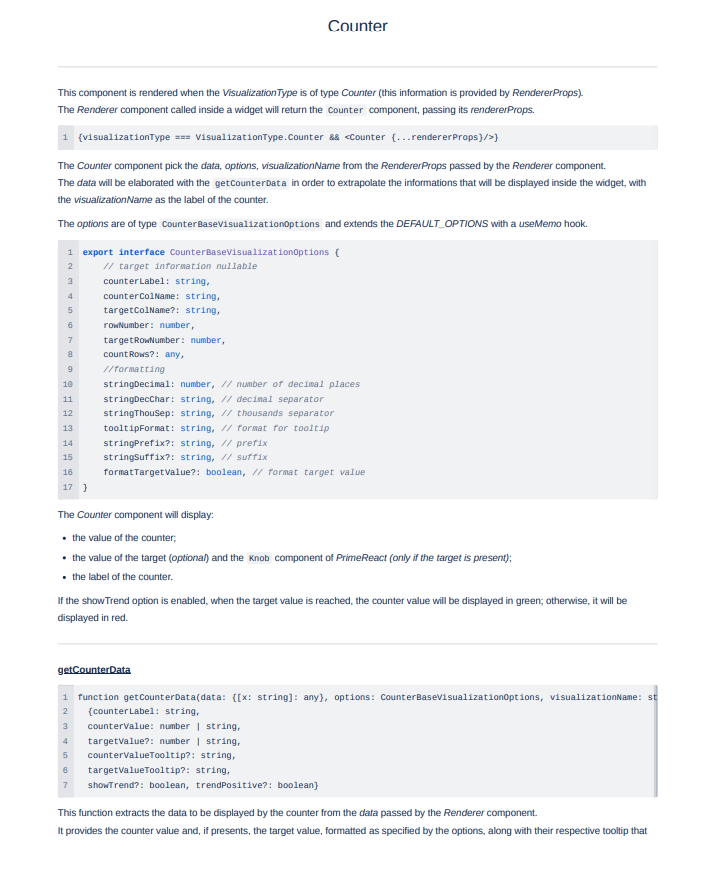
\includegraphics[alt={Esempio documentazione Confluence}, width=1 \textwidth]{img/ex_confluence.png}
    \caption{Esempio documentazione Confluence}
    \label{fig:ex_confluence}
\end{figure}

La documentazione è stata strutturata in modo da essere facilmente consultabile e comprensibile, con l'obiettivo di
fornire un supporto efficace agli sviluppatori futuri che potrebbero dover utilizzare la libreria. \newline
La produzione di una buona documentazione ricopre infatti un ruolo fondamentale al fine di garantire la manutenibilità
del codice e la facilità di comprensione delle funzionalità offerte dalla libreria, in modo da ridurre i tempi di
apprendimento e di sviluppo necessari per gli utilizzi futuri del prodotto implementato.

\section{Testing}

\chapter{Rilascio}
\label{chap:rilascio}
In questa sezione viene presentato il rilascio del prodotto finale, presentando infine un esemptio di integrazione dell'SDK
all'interno di un prodotto Datasoil S.rl. operativo.

\section{Rilascio SDK}
Al fine di rilasciare un package, è necessario effettuare la \textit{build} del prodotto. \\
Per il processo di building del codice è stato utilizzato \textit{Rollup}, un bundler di moduli JavaScript che permette:
\begin{itemize}
    \item di creare bundle di moduli in formato \textit{ESM} (ECMAScript Module) e \textit{CJS} (CommonJS);
    \item di utilizzare TypeScript all'interno del progetto, integrando la configurazione dichiarata nel file \textit{tsconfig.json};
    \item la risoluzione delle dipendenze tra i moduli, escludendo le \textit{peerdependency} dal bundle;
    \item la produzione di bundle di dimensioni ridotte grazie alla sua capacità di effettuare il tree-shaking;
    \item il supporto al plugin \textit{terser}, utilizzato per la minimizzazione del codice prodotto attraverso la rimozione dei commenti e degli spazi vuoti,
          effettuando il \textit{munging} dei nomi delle variabili e introducendo ottimizzazioni per ridurre la dimensione finale;
    \item il supportare a \textit{sourcemaps} per facilitare il debug del codice, permettendo di mappare il codice minificato con il codice sorgente originale;
    \item la generazione di file di dichiarazione TypeScript;
    \item il supporto a plugin per il calcolo della dimensione del bundle, specificando la dimensione di ogni singola dipendenze
          all'interno del progetto, generando un file di report \textit{html}.
\end{itemize}
Per effettuare la build del progetto è necessario eseguire il comando \textit{yarn build-package} configurato all'interno del file \textit{package.json} del progetto:
tale comando, come mostrato nel listato \ref{listing:scripts_package_json_dsdashboard2}, effettua la build del progetto, generando i file di output all'interno della cartella \textit{dist}.\\
Data la configurazione all'interno del file \textit{rollup.config.js}, il comando effettua la build del progetto in formato \textit{ESM} e \textit{CJS}.\\
Per specificare il punto di ingresso per i consumatori dei package, sono state definite all'interno del file \textit{package.json} le chiavi \textit{main} e \textit{module} che puntano
rispettivamente ai file \textit{dist/cjs/index.js} e \textit{dist/esm/index.esm.js}.
Utilizzando \textit{Yarn}, il rilascio di un package può avvenire principalmente tramite tre modalità differenti:
\begin{itemize}
    \item \textbf{Registro di npm}: è il registro di default di \textit{Yarn}, un registro pubblico che permette a chiunque abbiano
          un account di pubblicare pacchetti. Per impostazione predefinita (ma comunque configurabile), i pacchetti pubblicati su \textit{npm}
          sono visibili a tutti e di conseguenza tutti possono usufruirne;
    \item \textbf{Registro privato}: è un registro privato che permette di pubblicare pacchetti in un ambiente accessibile solo a chi è
          autorizzato. Esistono differenti servizi che offrono registri privati, a seconda del contesto operativo e delle esigenze dei prodotti
          che devono usufruire di tali pacchetti;
    \item \textbf{Github Packages}: è un \textit{software package hosting service} offerto da \textit{Github} che permette di pubblicare pacchetti
          in modo pubblico o privato all'interno di un repository \textit{Github}, come se fosse un registro \textit{npm}.
\end{itemize}
Per questo progetto è stato scelto di utilizzare quest'ultima opzione come registro di pubblicazione dei pacchetti, in quanto
all'interno di Datsoil S.r.l. i package prodotti vengono pubblicati all'interno dello spazio \textit{Github Packages} dell'organizzazione aziendale:
questo servizio è infatti molto utile per chi utilizza \textit{Github} come sistema di versionamento e vuole mantenere i pacchetti all'interno del proprio repository.
Per pubblicare un pacchetto all'interno di \textit{Github Packages} è necessario configurare il file \textit{package.json} del progetto, specificando
il campo \textit{publishConfig} nel seguente modo:

\begin{listing}[H]
    \begin{minted}{json}
    {
        "publishConfig": {
            "registry": "https://npm.pkg.github.com/"
        }
    }
    \end{minted}
    \caption{Configurazione del campo \textit{publishConfig} all'interno del file \textit{package.json}}
    \label{listing:package_json_publish_config}
\end{listing}

In seguito, dopo aver configurato il file \textit{.npmrc} all'interno del progetto, specificando il token di autenticazione per l'accesso al registro di \textit{Github Packages},
è possibile eseguire il comando \textit{yarn publish} per pubblicare il pacchetto: una volta avviato il comando, verrà illustrata la versione precedente del
package e verrà richiesto di fornirne una nuova. \\
Una volta terminato il processo di pubblicazione, il pacchetto sarà disponibile all'interno del registro di \textit{Github Packages} dell'organizzazione aziendale.

\section{Integrazione SDK all'interno di SYNMGR}
Durante lo svolgimento dello stage, ho avuto la possibilità di integrare l'SDK prodotto all'interno del prodotto \textit{SYNMGR} di Datasoil S.r.l.,
applicazione web di test utilizzata dall'azienda per testare gli sviluppi futuri e le nuove funzionalità che verranno in seguito rilasciate sul prodotto ufficiale \textit{SYN}. \\
Per utilizzare l'SDK all'interno di \textit{SYNMGR}, è stato necessario configurare il file \textit{.npmrc} all'interno del progetto, specificando il token di autenticazione
per l'accesso al registro di \textit{Github Packages}: utilizzando infatti il registro fornito da \textit{Github}, i package manager come \textit{Yarn} e \textit{npm} andranno
a verificare la presenza di tali informazioni e, solo nel caso di riscontro positivo, permetteranno l'installazione dei pacchetti. \\
In seguito, è stata sostituito il precedente SDK \textit{dsdashboard} a favore del nuovo SDK \textit{dsdashboard2} all'interno del file \textit{package.json} del progetto.

\begin{listing}[H]
    \begin{minted}{json}
    {
        "dependencies": {
            "@datasoil/dsdashboard2": "^0.1.5"
        }
    }
    \end{minted}
    \caption{Configurazione del campo \textit{dependencies} all'interno del file \textit{package.json} di \textit{SYNMGR}}
    \label{listing:package_json_synmgr}
\end{listing}

In seguito, è stato eseguito il comando \textit{yarn install} per installare il pacchetto all'interno del progetto, permettendo di utilizzare le nuove implementazioni delle
componenti inerenti alle dashboard.

\begin{figure}[H]
    \centering
    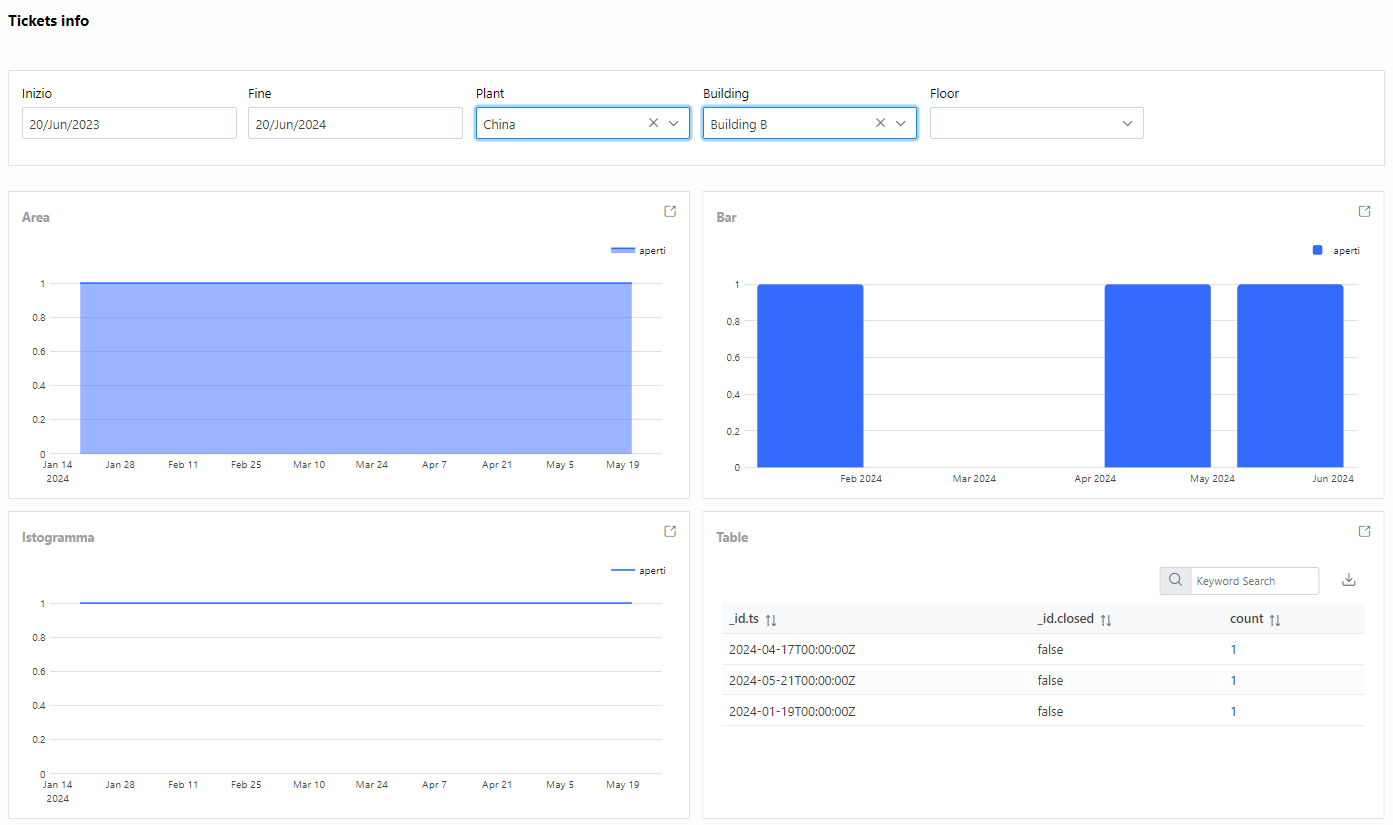
\includegraphics[alt={Esempio di dashboard all'interno di SYNMGR}, width=1 \columnwidth]{img/synmgr-dashboard.png}
    \caption{Esempio di dashboard all'interno di SYNMGR}
    \label{fig:synmgr_dashboard}
\end{figure}
\chapter{Conclusioni}
\label{chap:conclusioni}

\section{Valutazione del progetto}

\section{Riflessioni finali}

\section{Possibili Sviluppi futuri}

\backmatter
\pagenumbering{roman}
\chapter{Bibliografia}
\label{cap:bibliography}

\nocite{*}

% % Books bibliography
% \printbibliography[heading=subbibliography, title={Testi}, type=book]

% % Articles bibliography
% \printbibliography[heading=subbibliography, title={Articoli}, type=article]

% Websites bibliography
\printbibliography[heading=subbibliography, title={Siti}, type=online]

\chapter{Sitografia}
\label{cap:webliography}
\nocite{*}

% Websites bibliography
\printbibliography[heading=subbibliography, title={\null}, type=online]

\end{document}